% EDA / CAD technical interview | technology mapping and ECO
% English Beamer interview deck, expanded from user-authored ABC Mapper slides.
% Standalone Beamer source: pdfLaTeX, no external image files required.
% Mapping content preserved; ECO pages are clearly marked as proposed.
% NeoPower is a company project: keep discussion high-level and do not imply that
% every current repository module was personally authored during employment.
%
% Original mapping sequence:
%  1 Cover                 2 Education & Experience   3 Outline
%  4 ABC: Extension       5 ABC: Testing
%  6 NeoPower: Systems    7 NeoPower: Reliability
%  8 Thank You

\documentclass[aspectratio=169,10pt]{beamer}
\usepackage[english]{babel}
\usepackage[utf8]{inputenc}
\usepackage[T1]{fontenc}
\usepackage{lmodern}
\usepackage{amsmath,amssymb}
\usepackage{booktabs}
\usepackage{graphicx}
\usepackage{xcolor}
\usepackage{tikz}
\usetikzlibrary{arrows.meta,positioning,calc,shapes.geometric}
\usepackage{hyperref}
\graphicspath{{./}{figures/}}

% --------- Same Madrid-inspired visual identity as the ABC Mapper deck ---------
\usetheme{Madrid}
\usecolortheme{default}
\definecolor{Ink}{HTML}{243748}
\definecolor{Muted}{HTML}{667B8B}
\definecolor{Accent}{HTML}{347E74}
\definecolor{AccentBlue}{HTML}{507DAD}
\definecolor{SoftMint}{HTML}{E6F4EE}
\definecolor{SoftBlue}{HTML}{E9F2F9}
\definecolor{SoftLilac}{HTML}{F1EEF8}
\definecolor{Paper}{HTML}{FBFCFE}
\definecolor{Divider}{HTML}{D8E4EB}
\setbeamercolor{background canvas}{bg=Paper}
\setbeamercolor{normal text}{fg=Ink}
\setbeamercolor{structure}{fg=Accent}
\setbeamercolor{frametitle}{fg=Ink,bg=SoftBlue}
\setbeamercolor{title}{fg=Ink}
\setbeamercolor{subtitle}{fg=Muted}
\setbeamercolor{block title}{fg=Ink,bg=SoftBlue}
\setbeamercolor{block body}{fg=Ink,bg=white}
\setbeamercolor{item}{fg=Accent}
\setbeamercolor{footline}{fg=Muted,bg=Paper}
\setbeamercolor{panelblue}{fg=Ink,bg=SoftBlue!60}
\setbeamercolor{panelmint}{fg=Ink,bg=SoftMint!72}
\setbeamercolor{panellilac}{fg=Ink,bg=SoftLilac!76}
\setbeamercolor{panelwhite}{fg=Ink,bg=white}
\setbeamerfont{frametitle}{size=\Large,series=\bfseries}
\setbeamerfont{footline}{size=\tiny}
\setbeamertemplate{headline}{}
\setbeamertemplate{navigation symbols}{}
\setbeamertemplate{blocks}[rounded][shadow=false]
\setbeamertemplate{itemize items}[circle]
\setbeamertemplate{footline}{%
  \leavevmode\hbox{%
    \begin{beamercolorbox}[wd=\paperwidth,ht=.30cm,dp=.16cm,rightskip=.60cm plus 1fil]{footline}%
      \hfill\insertframenumber\,/\,\inserttotalframenumber
    \end{beamercolorbox}}%
}
\setbeamertemplate{frametitle}{%
  \nointerlineskip
  \begin{beamercolorbox}[wd=\paperwidth,ht=.77cm,dp=.18cm,leftskip=.64cm]{frametitle}%
    \usebeamerfont{frametitle}\insertframetitle
  \end{beamercolorbox}%
}

% --------- Same basic components, plus lightweight reusable panels ---------
\newcommand{\smalllabel}[1]{{\scriptsize\bfseries\color{Accent}\MakeUppercase{#1}}}
\newcommand{\takeaway}[1]{%
  \begin{beamercolorbox}[rounded=true,sep=0.15cm,wd=\linewidth]{block title}%
    \strut\textbf{#1}\strut
  \end{beamercolorbox}%
}
\newcommand{\minibadge}[2]{%
  \tikz[baseline=(badge.base)]\node[fill=#1,rounded corners=3pt,
    inner xsep=6pt,inner ysep=3pt] (badge) {\scriptsize\bfseries #2};%
}
\newcommand{\softpanel}[3]{%
  \begin{beamercolorbox}[rounded=true,sep=0.16cm,wd=\linewidth]{#1}%
    {\small\bfseries\color{Accent}#2}\par\vspace{0.08cm}
    {\small\color{Ink}#3}%
  \end{beamercolorbox}%
}
\newcommand{\smallpanel}[3]{%
  \begin{beamercolorbox}[rounded=true,sep=0.13cm,wd=\linewidth]{#1}%
    {\small\bfseries\color{Accent}#2}\par\vspace{0.06cm}
    {\scriptsize\color{Ink}#3}%
  \end{beamercolorbox}%
}
\newcommand{\outlinecard}[4]{%
  \begin{beamercolorbox}[rounded=true,sep=0.17cm,wd=\linewidth]{#1}%
    \begin{minipage}[c]{0.34\linewidth}
      {\normalsize\bfseries #2}\par\vspace{0.03cm}
      {\scriptsize\color{Accent}#3}
    \end{minipage}\hfill%
    \begin{minipage}[c]{0.63\linewidth}
      {\small #4}
    \end{minipage}%
  \end{beamercolorbox}%
}
\newcommand{\gate}[3]{%
  \begin{beamercolorbox}[rounded=true,sep=0.15cm,wd=\linewidth]{panelwhite}%
    {\small\bfseries\color{Accent}#1\quad #2}\par\vspace{0.07cm}
    {\scriptsize\color{Muted}#3}%
  \end{beamercolorbox}%
}


% --- Custom slide components: same color palette and structure as the template ---
% Reserved image areas can be replaced by \\includegraphics[width=...]{your_image}.
\newcommand{\figurespace}[3]{%
  \begin{tikzpicture}
    \node[draw=AccentBlue!50,dashed,rounded corners=3pt,fill=white,
      text width=.90\linewidth,minimum height=#1,align=center,inner sep=5pt] {%
      {\scriptsize\bfseries\color{AccentBlue}FIGURE SPACE}\\[3mm]
      {\normalsize\bfseries\color{Muted}#2}\\[2mm]
      {\scriptsize\color{Muted}#3}%
    };
  \end{tikzpicture}%
}
\newcommand{\statcard}[2]{%
  \begin{beamercolorbox}[rounded=true,sep=.13cm,wd=\linewidth]{panelwhite}
    {\Large\bfseries\color{Ink}#1}\par
    {\scriptsize\color{Muted}#2}
  \end{beamercolorbox}%
}
\newcommand{\scitem}[2]{%
  \begin{beamercolorbox}[rounded=true,sep=.14cm,wd=\linewidth]{panelblue}
    {\small\bfseries\color{Accent}#1}\par\vspace{.06cm}
    {\scriptsize #2}
  \end{beamercolorbox}%
}

% Reusable visual placeholder from the original portfolio template.
% Mapping / ECO research figures elsewhere in this deck continue to use \figurespace.
\providecommand{\aiplaceholder}[3]{}
\renewcommand{\aiplaceholder}[3]{%
  \par\noindent
  \begin{tikzpicture}
    \node[draw=AccentBlue!55,dashed,line width=0.6pt,
      rounded corners=4pt,fill=SoftBlue!35,
      text width=\dimexpr\linewidth-0.82cm\relax,
      minimum height=#1,inner xsep=0.40cm,inner ysep=0.12cm,
      outer sep=0pt,align=center] {%
      {\small\bfseries\color{AccentBlue}IMAGE PLACEHOLDER}\par
      \vspace{0.12cm}
      {\small\color{Ink}#2\par}
      \vspace{0.10cm}
      {\scriptsize\ttfamily\color{Muted}\detokenize{#3}\par}%
    };
  \end{tikzpicture}\par
}


\title[CAD Technical Interview]{EDA / CAD Engineering Projects}
\subtitle{Selected Research and Engineering Projects}
\author{Yu-Jui (Stanley) Liang}
\institute{National Taiwan University}
\date{}
% This document numbers every slide source block. To jump to a page,
% search for "SLIDE NN / 17" (for example "SLIDE 05 / 17").

% Unified S1-S5 card height; keeps five candidates easy to compare.
\newcommand{\ecostrategycard}[3]{%
  \begin{beamercolorbox}[rounded=true,sep=.20cm,wd=\linewidth]{#1}%
    \begin{minipage}[c][1.43cm][c]{\dimexpr\linewidth-.40cm\relax}
      {\normalsize\bfseries\color{Accent}#2}\par\vspace{.11cm}
      {\small\raggedright\hyphenpenalty=10000\exhyphenpenalty=10000 #3\par}
    \end{minipage}%
  \end{beamercolorbox}%
}

\begin{document}
% 15-minute shortlist: 6 mapping pages, 5 ECO pages, a contest title page.


% ============================================================
% No duplicate project listing on this cover; see slide 4.
% ============================================================
% ------------------------------------------------------------------------
% SLIDE 1 / 16 | Portfolio Cover
% ------------------------------------------------------------------------
{\setbeamertemplate{footline}{}
\begin{frame}[plain]
  \vspace*{1.65cm}
  \smalllabel{CAD Engineering Technical Interview}\par
  \vspace{0.51cm}
  {\raggedright\fontsize{21}{27}\selectfont\bfseries\color{Ink}
    EDA / CAD Engineering Projects\par}
  \vspace{0.29cm}
  {\normalsize\color{Muted}Logic Synthesis \enspace / \enspace Physical Design \enspace / \enspace Timing ECO \enspace / \enspace CAD Flow Automation\par}
  \vspace{0.70cm}
  {\Large\bfseries\color{Ink}Yu-Jui (Stanley) Liang}\par
  \vspace{0.10cm}
  {\normalsize\color{Muted}M.S. Candidate, Data Science Master Degree Program\par}
  {\normalsize\color{Muted}National Taiwan University\par}
  \vskip0pt plus 1filll
  {\color{Accent}\rule{\textwidth}{0.7pt}}\par
  \vspace{0.16cm}
  {\small\href{mailto:liangyujui@gmail.com}{liangyujui@gmail.com}
     \quad | \quad
     \href{https://www.linkedin.com/in/yu-jui-liang-735a57316}{linkedin.com/in/yu-jui-liang-735a57316}\par}
  \vspace*{0.55cm}
\end{frame}}

% ============================================================
% ============================================================
% ------------------------------------------------------------------------
% SLIDE 2 / 16 | Education & Research Interests
% ------------------------------------------------------------------------
\begin{frame}{Education \& Research Interests}
  \vspace{0.05cm}
  \smalllabel{01 / Profile}\par\vspace{0.10cm}
  \vfill
  \begin{columns}[T,onlytextwidth]
    \begin{column}{0.49\textwidth}
      \begin{beamercolorbox}[rounded=true,sep=0.20cm,wd=\linewidth]{panelblue}
        {\large\bfseries\color{AccentBlue}Education}\par
        \vspace{0.14cm}
        {\normalsize\bfseries National Taiwan University}\par
        {\normalsize M.S. Candidate, Data Science Master Degree Program}\par
        {\small\color{Muted}Sep. 2025 -- Expected Jun. 2027}\par
        \vspace{0.23cm}
        {\normalsize\bfseries National Chengchi University}\par
        {\normalsize B.S. in Computer Science}\par
        {\normalsize Double Major in Electronic Physics}\par
        {\small\color{Muted}Sep. 2021 -- Jun. 2025}
      \end{beamercolorbox}
    \end{column}
    \begin{column}{0.49\textwidth}
      \begin{beamercolorbox}[rounded=true,sep=0.20cm,wd=\linewidth]{panelmint}
        {\large\bfseries\color{Accent}Research Interests}\par
        \vspace{0.15cm}
        {\normalsize\bfseries EDA / CAD \& VLSI Design Automation}\par
        \vspace{0.09cm}
        {\normalsize Logic Synthesis}\par
        {\normalsize Technology Mapping}\par
        {\normalsize Static Timing Analysis}\par
        {\normalsize Timing Closure}\par
        {\normalsize Physical Design}\par
        {\normalsize Incremental ECO}\par
        {\normalsize PPA}\par
        \vspace{0.15cm}
        {\normalsize\bfseries Algorithm \& Software Development}\par
        \vspace{0.09cm}
        {\normalsize C++ / Python / Tcl Flow Automation}\par
      \end{beamercolorbox}
    \end{column}
  \end{columns}
  \vfill
\end{frame}

% ============================================================
% ============================================================
% ------------------------------------------------------------------------
% SLIDE 3 / 16 | Professional Software Engineering Experience
% ------------------------------------------------------------------------
\begin{frame}{Professional Software Engineering Experience}
  \vspace{0.04cm}
  \smalllabel{02 / Work Experience}\par\vspace{0.10cm}
  \takeaway{Software development, simulation, and validation experience in R\&D environments.}
  \vfill

  \begin{beamercolorbox}[rounded=true,sep=0.19cm,wd=\linewidth]{panelblue}
    {\normalsize\bfseries\color{Ink}AIMobile Co., Ltd. (Inventec Group)}\hfill
    {\scriptsize\color{Muted}Apr. 2025 -- Jul. 2025}\par
    \vspace{0.07cm}
    {\small\bfseries\color{AccentBlue}Contract Software Engineer}\par
    \vspace{0.14cm}
    {\small\color{Ink}Contributed to software development and system integration in an R\&D environment.}\par
    \vspace{0.08cm}
    {\small\color{Ink}Supported debugging and functional validation across software modules.}\par
  \end{beamercolorbox}

  \vfill
  \begin{beamercolorbox}[rounded=true,sep=0.19cm,wd=\linewidth]{panelmint}
    {\normalsize\bfseries\color{Ink}Neopower Technologies Co., Ltd.}\hfill
    {\scriptsize\color{Muted}Jun. 2023 -- Mar. 2025}\par
    \vspace{0.07cm}
    {\small\bfseries\color{Accent}Contract Software Engineer}\par
    \vspace{0.14cm}
    {\small\color{Ink}Developed a custom system simulator to reproduce operational and error scenarios.}\par
    \vspace{0.08cm}
    {\small\color{Ink}Performed regression checks, log analysis, and customer-side A/B validation.}\par
  \end{beamercolorbox}
  \vfill
\end{frame}

% ============================================================
% ============================================================
% ------------------------------------------------------------------------
% SLIDE 4 / 16 | Selected Projects & Discussion Topics
% ------------------------------------------------------------------------
\begin{frame}{Selected Projects \& Discussion Topics}
  \vspace{0.03cm}
  \smalllabel{03 / Project Overview}\par\vspace{0.11cm}
  \vfill
  \begin{beamercolorbox}[rounded=true,sep=0.20cm,wd=\linewidth]{panelblue}
    {\small\bfseries\color{AccentBlue}01 \quad Master's Research --- Logic Synthesis (Front End)}\par
    \vspace{0.05cm}
    {\normalsize\bfseries Joint Single- and Multi-Output Cell Mapping\\via Differentiable Optimization}\par
    \vspace{0.07cm}
    {\small EDA Tool Development \quad / \quad Boolean Matching \quad / \quad Area--Delay Optimization}
  \end{beamercolorbox}
  \vfill
  \begin{beamercolorbox}[rounded=true,sep=0.20cm,wd=\linewidth]{panellilac}
    {\small\bfseries\color{Accent}02 \quad ICCAD 2025 Problem C --- CAD Methodology (Back End)}\par
    \vspace{0.05cm}
    {\normalsize\bfseries STA-Driven Incremental Timing ECO Search}\par
    \vspace{0.07cm}
    {\small OpenROAD / OpenSTA \quad / \quad Python--Tcl Flow Automation \quad / \quad Heuristic PPA Search}
  \end{beamercolorbox}
  \vfill
\end{frame}

% ==============================================================
% Main technical contents retained from the uploaded Beamer source.
% The 15-minute and 30-minute versions allocate equal time to
% Project 01 (Mapping) and Project 02 (STA-Driven ECO Optimization).
% ==============================================================

% ------------------------------------------------------------------------
% SLIDE 5 / 16 | Project Overview: NF-Direct MO Mapping
% ------------------------------------------------------------------------
\begin{frame}[shrink=8]{Project Overview: NF-Direct MO Mapping}
  \vspace{.02cm}
  \smalllabel{01 / Research Scope}\par\vspace{.10cm}
  \takeaway{Discover FA/HA opportunities and globally pre-select MO candidates before GradMap.}
  \vspace{.18cm}
  \begin{columns}[T,onlytextwidth]
    \begin{column}{.47\textwidth}
      \smallpanel{panelblue}{Problem}{Single-output cut retention does not explicitly optimize two-output FA/HA opportunities.}
      \vspace{.15cm}
      \smallpanel{panelmint}{Our Extension}{Add independent NF-direct MO discovery inside ABC \texttt{\&nf}, without changing SO mapping.}
      \vspace{.15cm}
      \smallpanel{panellilac}{Proposed Optimization}{Solve an area-aware non-overlapping MO selection MILP before GradMap.}
    \end{column}
    \begin{column}{.48\textwidth}
      \minibadge{SoftMint}{Research Pipeline}\par\vspace{.13cm}
      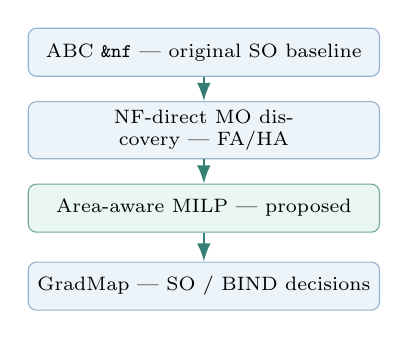
\begin{tikzpicture}[>=Latex,font=\scriptsize]
      \tikzset{b/.style={draw=AccentBlue!60,fill=SoftBlue!85,rounded corners=3pt,text width=4.25cm,minimum height=.61cm,align=center,inner sep=3pt},
                m/.style={b,draw=Accent!70,fill=SoftMint!82}}
      \node[b] (nf) at (0,0) {ABC \texttt{\&nf} — original SO baseline};
      \node[b] (mo) at (0,-.99) {NF-direct MO discovery — FA/HA};
      \node[m] (ilp) at (0,-1.98) {Area-aware MILP — proposed};
      \node[b] (grad) at (0,-2.97) {GradMap — SO / BIND decisions};
      \foreach \a/\b in {nf/mo,mo/ilp,ilp/grad} {\draw[->,Accent,thick](\a.south)--(\b.north);}
      \end{tikzpicture}
      \par\vspace{.05cm}
      {\scriptsize\color{Muted}Input AIG + Liberty $\rightarrow$ selected.matches $\rightarrow$ mapped netlist}
    \end{column}
  \end{columns}
\end{frame}


% ------------------------------------------------------------------------
% SLIDE 6 / 16 | Why an Independent MO Discovery Path?
% ------------------------------------------------------------------------
\begin{frame}[shrink=3]{Why an Independent MO Discovery Path?}
  \vspace{.02cm}\smalllabel{03 / Motivation}\par\vspace{.08cm}
  \takeaway{SO-oriented cut pruning may remove cuts useful for joint FA/HA output matching.}
  \vspace{.19cm}
  \begin{columns}[T,onlytextwidth]
    \begin{column}{.45\textwidth}
      \softpanel{panelblue}{Original NF SO Cut Ranking}{Cuts are retained according to single-output objectives, not complementary FA/HA output pairs.}
      \vspace{.22cm}
      \softpanel{panelmint}{Independent NF-Direct Sidecar}{Propagate additional MO cuts and CON/SN truth projections without modifying NF's SO path.}
    \end{column}
    \begin{column}{.52\textwidth}
      \figurespace{3.24cm}{SO-pruned cut vs MO-retained cut}{Two output roots with a shared legal 3-leaf input support.}
    \end{column}
  \end{columns}
  \vspace{.20cm}
  {\small\bfseries\color{Accent}MO discovery is not equivalent to scanning the final selected SO cover.}
\end{frame}


% ------------------------------------------------------------------------
% SLIDE 7 / 16 | NF-Direct MO Candidate Discovery
% ------------------------------------------------------------------------
\begin{frame}[shrink=9]{NF-Direct MO Candidate Discovery}
  \vspace{.02cm}\smalllabel{04 / Core Algorithm}\par\vspace{.08cm}
  \takeaway{Pair compatible CON and SN projections over a common input support.}
  \vspace{.18cm}
  \begin{columns}[T,onlytextwidth]
    \begin{column}{.45\textwidth}
      \scitem{01 / MO Cut Propagation}{Independent retention of FA/HA-relevant truth functions and supports.}
      \vspace{.16cm}
      \scitem{02 / Projection Pairing}{Match CON / SN roles using shared leaves, permutation and phase.}
      \vspace{.16cm}
      \scitem{03 / Legality + Witness}{Validate the pair and export v3 MOCAND records with replacement roots.}
    \end{column}
    \begin{column}{.52\textwidth}
      \figurespace{3.38cm}{Example: FA CON / SN cut projections}{Highlight two output roots, same leaves, shared cell configuration.}
      \vspace{.11cm}
      \minibadge{SoftMint}{OUTPUT: BIND / ROOTS / FANINS / REPLACE\_ROOTS}
    \end{column}
  \end{columns}
\end{frame}


% ------------------------------------------------------------------------
% SLIDE 8 / 16 | Baseline: File-Order Candidate Loss
% ------------------------------------------------------------------------
\begin{frame}[shrink=8]{Baseline: File-Order Candidate Loss}
  \vspace{.02cm}\smalllabel{08 / Motivation for MILP}\par\vspace{.08cm}
  \takeaway{File-order greedy filtering ignores estimated area benefits of conflicting MO candidates.}
  \vspace{.17cm}
  \begin{columns}[T,onlytextwidth]
    \begin{column}{.319\textwidth}\statcard{41,476}{Original MO candidate BIND records}\end{column}
    \begin{column}{.319\textwidth}\statcard{7,024}{FIFO retained (offline simulation)}\end{column}
    \begin{column}{.319\textwidth}\statcard{16.9\%}{Overall retention rate}\end{column}
  \end{columns}
  \vspace{.07cm}
  \begin{center}
  \footnotesize
\begin{tabular}{@{}lrrrr@{}}
\toprule
\textbf{Design} & \textbf{Original MO} & \textbf{FIFO Retained} & \textbf{Dropped} & \textbf{Retention} \\
\midrule
EPFL hyp & 25,440 & 4,180 & 21,260 & 16.4\% \\
EPFL square & 3,658 & 544 & 3,114 & 14.9\% \\
EPFL log2 & 2,798 & 400 & 2,398 & 14.3\% \\
EPFL multiplier & 2,190 & 349 & 1,841 & 15.9\% \\
EPFL voter & 632 & 106 & 526 & 16.8\% \\
ISCAS c6288 & 258 & 37 & 221 & 14.3\% \\
ISCAS c7552 & 102 & 11 & 91 & 10.8\% \\
EPFL adder & 6 & 1 & 5 & 16.7\% \\
\textbf{All 364 designs} & \textbf{41,476} & \textbf{7,024} & \textbf{34,452} & \textbf{16.9\%} \\
\bottomrule
\end{tabular}
  \end{center}
  \vspace{-0.02cm}
  {\tiny\color{Muted}Source: NF-direct full-corpus census, 364 benchmark entries; simulated parser-policy first-fit, not trained GradMap QoR.}
\end{frame}


% ------------------------------------------------------------------------
% SLIDE 9 / 16 | Area-Aware MO Selection (MILP)
% ------------------------------------------------------------------------
\begin{frame}[shrink=15]{Area-Aware MO Selection (MILP)}
  \vspace{.02cm}\smalllabel{09 / Proposed Global Selection}\par\vspace{.08cm}
  \takeaway{Maximize estimated area savings subject to non-overlapping MO candidates.}
  \vspace{.13cm}
  \begin{columns}[T,onlytextwidth]
    \begin{column}{.59\textwidth}
      \begin{beamercolorbox}[rounded=true,sep=.12cm,wd=\linewidth]{panelwhite}
      {\small
      \[\boxed{\begin{aligned}
        \max\quad &\sum_{i=1}^{N}\bigl(A_i^{SO}-A_i^{MO}\bigr)x_i\\[4pt]
        \text{s.t.}\quad &\sum_{i=1}^{N} a_{vi}x_i\leq1,\quad\forall v\in\mathcal V\\[4pt]
        &x_i\in\{0,1\},\quad i=1,\ldots,N
      \end{aligned}}\]
      }
      \end{beamercolorbox}
      \vspace{.17cm}
      \smallpanel{panelblue}{Notation}{%
        $x_i$: select MO $i$; $A_i^{SO}$: SO witness area; $A_i^{MO}$: MO cell area;\\
        $a_{vi}=1$ iff AIG base node $v$ belongs to MO candidate $i$; otherwise $0$.}
    \end{column}
    \begin{column}{.38\textwidth}
      \figurespace{2.06cm}{Conflict: (A,B) vs (A,C)}{Shared AIG node A $\Rightarrow$ at most one MO selected.}
      \vspace{.15cm}
      \smallpanel{panelmint}{Implementation}{Python + HiGHS (\texttt{highspy}); emit selected.matches.}
    \end{column}
  \end{columns}
  \vspace{.12cm}
  {\scriptsize\color{Muted}Objective weights estimate local SO-to-MO benefits; actual GradMap final mapped area is measured later.}
\end{frame}


% ------------------------------------------------------------------------
% SLIDE 10 / 16 | Research Status & Next Steps
% ------------------------------------------------------------------------
\begin{frame}[shrink=5]{Research Status \& Next Steps}
  \vspace{.02cm}\smalllabel{11 / Outlook}\par\vspace{.08cm}
  \takeaway{Verified NF-direct discovery today; area-aware MILP is the next research step.}
  \vspace{.23cm}
  \begin{columns}[T,onlytextwidth]
    \begin{column}{.48\textwidth}
      \begin{beamercolorbox}[rounded=true,sep=.23cm,wd=\linewidth]{panelblue}
        {\normalsize\bfseries\color{Accent}Completed / Verified}\par\vspace{.16cm}
        {\small
        $\bullet$ Independent NF-direct MO discovery\\[1mm]
        $\bullet$ Boolean / structural legality\\[1mm]
        $\bullet$ SO witness + MOCAND integration\\[1mm]
        $\bullet$ 364-design candidate census}
      \end{beamercolorbox}
    \end{column}
    \begin{column}{.48\textwidth}
      \begin{beamercolorbox}[rounded=true,sep=.23cm,wd=\linewidth]{panelmint}
        {\normalsize\bfseries\color{Accent}Next / Proposed}\par\vspace{.16cm}
        {\small
        $\bullet$ Estimate SO witness area weights\\[1mm]
        $\bullet$ Solve MO selection with HiGHS\\[1mm]
        $\bullet$ Compare FIFO versus MILP\\[1mm]
        $\bullet$ Evaluate final mapped area / CEC}
      \end{beamercolorbox}
    \end{column}
  \end{columns}
  \vspace{.33cm}
  \begin{beamercolorbox}[rounded=true,sep=.19cm,wd=\linewidth]{panelwhite}
    {\scriptsize\bfseries\color{Accent}Research question}\par\vspace{.08cm}
    {\small\bfseries Can area-aware global pre-selection improve the MO opportunities available to GradMap?}
  \end{beamercolorbox}
  \vfill
  {\scriptsize\color{Muted}QoR results intentionally left pending until the new code and benchmark runs are complete.}
\end{frame}



% ============================================================
% PROJECT 02 SECTION OPENER | simplified ICCAD 2025 Problem C
% ============================================================
% ------------------------------------------------------------------------
% SLIDE 11 / 16 | Project 02 Opener: ICCAD 2025 CAD Contest Problem C
% ------------------------------------------------------------------------
{\setbeamertemplate{footline}{}
\begin{frame}[plain]
  \vfill
  \smalllabel{Project 02 / ICCAD 2025 CAD Contest / Problem C}\par
  \vspace{.40cm}
  \begin{beamercolorbox}[rounded=true,sep=.25cm,wd=\linewidth]{panelblue}
    {\fontsize{13.6}{17}\selectfont\bfseries\color{Ink}
    \mbox{Incremental Placement Optimization Beyond Detailed Placement}\par}
    \vspace{.14cm}
    {\normalsize\color{Ink}
      Simultaneous Gate Sizing, Buffering, and Cell Relocation\par}
  \end{beamercolorbox}
  \vspace{.80cm}
  \smalllabel{My Proposed Approach}\par
  \vspace{.17cm}
  {\fontsize{18}{23}\selectfont\bfseries\color{Accent}
    STA-Driven Incremental Timing ECO Search\par}
  \vspace{.18cm}
  {\small\color{Muted}
    Use OpenROAD / OpenSTA with policy-controlled ECO moves and global PPA evaluation.\par}
  \vfill
\end{frame}}
% ------------------------------------------------------------------------
% SLIDE 12 / 16 | Multi-Objective Timing ECO Optimization
% ------------------------------------------------------------------------
\begin{frame}{Multi-Objective Timing ECO Optimization}
  \vspace{.01cm}
  \smalllabel{02 / Problem Definition}\par\vspace{.10cm}
  \takeaway{Improve setup TNS toward zero while controlling total power, HPWL, and cell displacement.}
  \vspace{.14cm}

  % ---- Contest objectives: what matters after an ECO repair ----
  \smalllabel{Optimization Objectives}\par\vspace{.08cm}
  \begin{columns}[T,onlytextwidth]
    \begin{column}{.226\textwidth}
      \begin{beamercolorbox}[rounded=true,sep=.14cm,wd=\linewidth]{panelblue}
        {\small\bfseries\color{AccentBlue}01 / Setup TNS}\par\vspace{.11cm}
        {\scriptsize Reduce negative setup\par slack at violating endpoints.}
      \end{beamercolorbox}
    \end{column}
    \begin{column}{.226\textwidth}
      \begin{beamercolorbox}[rounded=true,sep=.14cm,wd=\linewidth]{panelmint}
        {\small\bfseries\color{Accent}02 / Total Power}\par\vspace{.11cm}
        {\scriptsize Avoid excess power\par from ECO changes.}
      \end{beamercolorbox}
    \end{column}
    \begin{column}{.226\textwidth}
      \begin{beamercolorbox}[rounded=true,sep=.14cm,wd=\linewidth]{panellilac}
        {\small\bfseries\color{AccentBlue}03 / HPWL}\par\vspace{.11cm}
        {\scriptsize Control estimated\par wirelength after ECO.}
      \end{beamercolorbox}
    \end{column}
    \begin{column}{.226\textwidth}
      \begin{beamercolorbox}[rounded=true,sep=.14cm,wd=\linewidth]{panelblue}
        {\small\bfseries\color{Accent}04 / Displacement}\par\vspace{.11cm}
        {\scriptsize Limit cell movement\par and keep placement legal.}
      \end{beamercolorbox}
    \end{column}
  \end{columns}

  \vspace{.13cm}
  % ---- Conceptual ECO pipeline, not the proposed branch-search algorithm ----
  \smalllabel{Basic ECO Evaluation Pipeline}\par\vspace{.09cm}
  \centering
  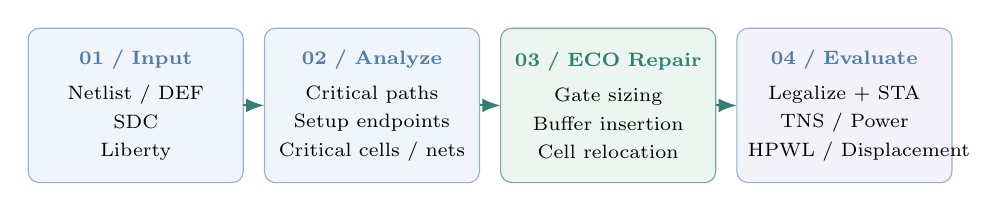
\begin{tikzpicture}[>=Latex,font=\scriptsize]
    \tikzset{
      ecoStage/.style={draw=AccentBlue!60,fill=SoftBlue!74,
        rounded corners=4pt,text width=2.45cm,minimum height=1.96cm,
        inner xsep=4pt,inner ysep=4pt,align=center,outer sep=0pt},
      ecoMint/.style={ecoStage,draw=Accent!68,fill=SoftMint!80},
      ecoLilac/.style={ecoStage,draw=AccentBlue!60,fill=SoftLilac!83}
    }
    \node[ecoStage] (input) at (0,0) {%
      {\bfseries\color{AccentBlue}01 / Input}\\[1.6mm]
      \mbox{Netlist / DEF}\\[.8mm]
      \mbox{SDC}\\[.8mm]
      \mbox{Liberty}};
    \node[ecoStage] (detect) at (3.00,0) {%
      {\bfseries\color{AccentBlue}02 / Analyze}\\[1.6mm]
      \mbox{Critical paths}\\[.8mm]
      \mbox{Setup endpoints}\\[.8mm]
      \mbox{Critical cells / nets}};
    \node[ecoMint] (repair) at (6.00,0) {%
      {\bfseries\color{Accent}03 / ECO Repair}\\[1.6mm]
      \mbox{Gate sizing}\\[.8mm]
      \mbox{Buffer insertion}\\[.8mm]
      \mbox{Cell relocation}};
    \node[ecoLilac] (evaluate) at (9.00,0) {%
      {\bfseries\color{AccentBlue}04 / Evaluate}\\[1.6mm]
      \mbox{Legalize + STA}\\[.8mm]
      \mbox{TNS / Power}\\[.8mm]
      {\fontsize{6.65}{8}\selectfont\mbox{HPWL / Displacement}}};
    \foreach \from/\to in {input/detect,detect/repair,repair/evaluate}{%
      \draw[->,Accent,thick] (\from.east)--(\to.west);}
  \end{tikzpicture}\par
  \vspace{.17cm}
  {\small\bfseries\color{Accent}Key challenge: a timing fix can worsen power or physical cost.\par}
\end{frame}

% ------------------------------------------------------------------------
% SLIDE 13 / 16 | Five Automatic ECO Strategy Candidates
% ------------------------------------------------------------------------
\begin{frame}{Five Automatic ECO Strategy Candidates}
  \vspace{.01cm}
  \smalllabel{02 / Candidate Set}\par\vspace{.12cm}
  \takeaway{The candidate is an automatic repair policy and editable region, not a manually chosen cell replacement.}
  \vspace{.37cm}
  \begin{columns}[T,onlytextwidth]
    \begin{column}{.32\textwidth}
      \ecostrategycard{panelblue}{S1 / Global Setup}{Whole design; automatic upsizing and VT selection.}
    \end{column}
    \begin{column}{.32\textwidth}
      \ecostrategycard{panelmint}{S2 / Path-Restricted}{Top-K path cells + nets; localized setup repair.}
    \end{column}
    \begin{column}{.32\textwidth}
      \ecostrategycard{panellilac}{S3 / Overlap-Aware}{Top-I shared cells, nets fixed; sizing / VT repair.}
    \end{column}
  \end{columns}
  \vspace{.34cm}
  \begin{columns}[T,onlytextwidth]
    \begin{column}{.49\textwidth}
      \ecostrategycard{panelmint}{S4 / Local Buffering}{Top-K nets, original cells fixed; buffer insertion and load splitting.}
    \end{column}
    \begin{column}{.49\textwidth}
      \ecostrategycard{panelblue}{S5 / Power Recovery}{Slack-rich cells / wider region; lower-power equivalent cells.}
    \end{column}
  \end{columns}
\end{frame}

% ------------------------------------------------------------------------
% SLIDE 14 / 16 | STA-Guided ECO Search: Best-First Branch List
% ------------------------------------------------------------------------
\begin{frame}{STA-Guided ECO Search: Best-First Branch List}
  \vspace{.01cm}\smalllabel{02 / Heuristic Search Policy}\par\vspace{.07cm}
  \takeaway{No better child this round? Continue from the best unexplored state in the Branch List.}
  \vspace{.13cm}
  \begin{columns}[T,onlytextwidth]
    \begin{column}{.585\textwidth}
      {\small\bfseries\color{Accent}Search Tree Example}\par\vspace{.08cm}
      \centering
      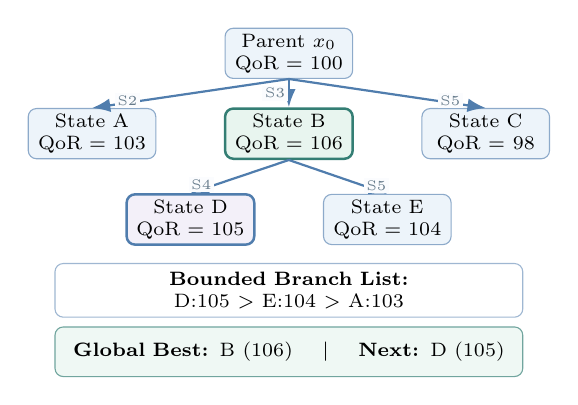
\begin{tikzpicture}[>=Latex,font=\scriptsize]
        \tikzset{
          state/.style={draw=AccentBlue!65,fill=SoftBlue!82,rounded corners=3pt,
            text width=1.48cm,minimum height=.57cm,align=center,inner sep=2pt},
          best/.style={state,draw=Accent,fill=SoftMint!92,line width=.9pt},
          next/.style={state,draw=AccentBlue,fill=SoftLilac!87,line width=.9pt},
          move/.style={font=\tiny,text=Muted,fill=Paper,inner sep=1pt}
        }
        \node[state] (root) at (2.64,0) {Parent $x_0$\\$\mathrm{QoR}=100$};
        \node[state] (a) at (.14,-1.02) {State A\\$\mathrm{QoR}=103$};
        \node[best] (b) at (2.64,-1.02) {State B\\$\mathrm{QoR}=106$};
        \node[state] (c) at (5.14,-1.02) {State C\\$\mathrm{QoR}=98$};
        \draw[->,AccentBlue,thick] (root.south) -- node[move,near end,left]{S2} (a.north);
        \draw[->,AccentBlue,thick] (root.south) -- node[move,midway,left]{S3} (b.north);
        \draw[->,AccentBlue,thick] (root.south) -- node[move,near end,right]{S5} (c.north);
        \node[next] (d) at (1.39,-2.11) {State D\\$\mathrm{QoR}=105$};
        \node[state] (e) at (3.89,-2.11) {State E\\$\mathrm{QoR}=104$};
        \draw[->,AccentBlue,thick] (b.south) -- node[move,near end,left]{S4} (d.north);
        \draw[->,AccentBlue,thick] (b.south) -- node[move,near end,right]{S5} (e.north);
        \node[draw=AccentBlue!55,fill=white,rounded corners=3pt,
          text width=5.73cm,minimum height=.57cm,align=center,inner sep=3pt]
          at (2.64,-3.01) {\textbf{Bounded Branch List:} D:105 $>$ E:104 $>$ A:103};
        \node[draw=Accent!70,fill=SoftMint!65,rounded corners=3pt,
          text width=5.73cm,minimum height=.63cm,align=center,inner sep=3pt]
          at (2.64,-3.79) {\textbf{Global Best:} B (106) \quad $\vert$ \quad
            \textbf{Next:} D (105)};
      \end{tikzpicture}
    \end{column}
    \begin{column}{.395\textwidth}
      {\small\bfseries\color{Accent}Heuristic Search Steps}\par\vspace{.12cm}
      \begin{beamercolorbox}[rounded=true,sep=.15cm,wd=\linewidth]{panelwhite}
        {\small\bfseries\color{Accent}01 / Pop Parent}\par
        {\scriptsize Highest-QoR unexplored state from the \textbf{Branch List}.}\par
        \vspace{.10cm}
        {\small\bfseries\color{Accent}02 / Generate + Evaluate}\par
        {\scriptsize STA-guided ECO moves, legalization, and global QoR score.}\par
        \vspace{.10cm}
        {\small\bfseries\color{Accent}03 / Update States}\par
        {\scriptsize Save improved \textbf{Global Best}; queue legal child states.}\par
        \vspace{.10cm}
        {\small\bfseries\color{Accent}04 / Next Branch}\par
        {\scriptsize Expand best branch, \textbf{even with no new Global Best}.}
      \end{beamercolorbox}
    \end{column}
  \end{columns}
  \vspace{.10cm}
  {\scriptsize\bfseries\color{Accent}A lower-scoring intermediate state may lead to a better ECO sequence later.}\par
\end{frame}

% ------------------------------------------------------------------------
% SLIDE 15 / 16 | QoR Results & Conclusion
% ------------------------------------------------------------------------
\begin{frame}{QoR Results \& Conclusion}
  \vspace{.01cm}\smalllabel{02 / Earlier ECO Evaluation}\par\vspace{.11cm}
  {\small\color{Muted}Setup-focused timing repair and the resulting power / wirelength trade-off.}\par
  \vspace{.08cm}
  \begin{columns}[T,onlytextwidth]
    \begin{column}{.49\textwidth}
      {\small\bfseries\color{Accent}Setup Timing}\par\vspace{.10cm}
      \begin{beamercolorbox}[rounded=true,sep=.14cm,wd=\linewidth]{panelblue}
        {\fontsize{24}{27}\selectfont\bfseries\color{AccentBlue}16.7\%}\par\vspace{.025cm}
        {\small\bfseries Median Setup TNS Improvement}\par
      \end{beamercolorbox}
      \vspace{.10cm}
      \begin{beamercolorbox}[rounded=true,sep=.14cm,wd=\linewidth]{panellilac}
        {\fontsize{24}{27}\selectfont\bfseries\color{AccentBlue}14.6\%}\par\vspace{.025cm}
        {\small\bfseries Average Setup WNS Improvement}\par
      \end{beamercolorbox}
    \end{column}
    \begin{column}{.49\textwidth}
      {\small\bfseries\color{Accent}Power \& Wirelength}\par\vspace{.10cm}
      \begin{beamercolorbox}[rounded=true,sep=.14cm,wd=\linewidth]{panelmint}
        {\fontsize{24}{27}\selectfont\bfseries\color{Accent}8\%}\par\vspace{.025cm}
        {\small\bfseries Total Power Reduction}\par
      \end{beamercolorbox}
      \vspace{.10cm}
      \begin{beamercolorbox}[rounded=true,sep=.14cm,wd=\linewidth]{panelblue}
        {\fontsize{24}{27}\selectfont\bfseries\color{Ink}+2\%}\par\vspace{.025cm}
        {\small\bfseries HPWL Increase}\par
      \end{beamercolorbox}
    \end{column}
  \end{columns}
  \vspace{.09cm}
  \begin{beamercolorbox}[rounded=true,sep=.13cm,wd=\linewidth]{panelwhite}
    {\small\bfseries\color{Accent}Conclusion}\par\vspace{.025cm}
    {\small\color{Ink}ECO operators can improve setup timing and power while accepting a small wirelength trade-off.}
  \end{beamercolorbox}
  \vspace{.06cm}
\end{frame}

% ------------------------------------------------------------------------
% SLIDE 16 / 16 | Thank You / Questions and Discussion
% ------------------------------------------------------------------------
{\setbeamertemplate{footline}{}
\begin{frame}[plain]
  \centering
  \vfill
  {\fontsize{36}{42}\selectfont\bfseries\color{Ink}THANK YOU}\par
  \vspace{.37cm}
  {\fontsize{19}{24}\selectfont\color{Muted}Questions \& Discussion}\par
  \vfill
\end{frame}}

\end{document}
